\documentclass[12pt,a4paper]{paper}
\usepackage[utf8]{inputenc}
\usepackage[english]{babel}
\usepackage{amsmath}
\usepackage{enumitem}
\usepackage{amsfonts}
\usepackage{amssymb}
\usepackage[left=1cm,right=1cm,top=1.5cm,bottom=2cm]{geometry}
\usepackage{Sweave}
\begin{document}
\title{STAT636 - Homework 2\\\small{Daniel Osorio - dcosorioh@tamu.edu\\Department of Veterinary Integrative Biosciences\\Texas A\&M University}}
\maketitle
\Sconcordance{concordance:STAT636_Template.tex:STAT636_Template.Rnw:%
1 8 1 1 0 6 1 1 2 1 0 3 1 6 0 2 1 8 0 1 2 10 1 1 2 4 0 1 2 1 1 1 2 1 0 %
1 1 5 0 6 1 4 0 2 2 1 0 1 1 5 0 6 1 4 0 2 2 9 0 1 2 2 1 1 2 4 0 1 2 2 1 %
1 2 1 0 1 4 7 0 1 3 1 0 1 1 4 0 1 2 9 1 4 0 1 3 2 1}

\begin{enumerate}
\item Find the maximum likelihood estimates of the 2 $\times$ 1 mean vector $\mu$ and the 2 $\times$ 2 covariance matrix $\Sigma$ based on the random sample
\[X = \left[\begin{array}{cc}3 & 6\\4 & 4\\5 & 7\\4 & 7\end{array}\right]\]
\begin{Schunk}
\begin{Sinput}
> X <- matrix(data = c(3,6,4,4,5,7,4,7), ncol = 2, byrow = TRUE)
> n <- nrow(X)
> X_hat <- 1/n * rep(1,n) %*% X
> X_hat
\end{Sinput}
\begin{Soutput}
     [,1] [,2]
[1,]    4    6
\end{Soutput}
\begin{Sinput}
> S_hat <- 1/n * (t(X) - drop(X_hat)) %*% t(t(X) - drop(X_hat))
> S_hat
\end{Sinput}
\begin{Soutput}
     [,1] [,2]
[1,] 0.50 0.25
[2,] 0.25 1.50
\end{Soutput}
\end{Schunk}
\item Let X$_{1}$, X$_{2}$, \dots, X$_{60}$ be a random sample of size n = 60 from a N$_{6}$($\mu$, $\Sigma$) population. Specify each of the following.
\begin{enumerate}
\item The distribution of $(X_{1} - \mu)'\Sigma^{-1}(X_{1} - \mu)$. \[(X_{1} - \mu)'\Sigma^{-1}(X_{1} - \mu) \sim \mathcal{X}^{2}_{6}\]
\item The distributions of $\bar{X}$ and $\sqrt{n}(\bar{X} - \mu)$.
\[\bar{X} \sim \mathcal{N}_{6}\left(\mu, \frac{1}{60}\Sigma \right)\]
\[\sqrt{n}(\bar{X} - \mu) \mathrel{\dot\sim} \mathcal{N}_{6}\left(0, \Sigma\right)\]
\item The distribution of $n(\bar{X}-\mu)'\Sigma^{-1}(\bar{X} - \mu)$ \[n(\bar{X}-\mu)'\Sigma^{-1}(\bar{X} - \mu) \sim \mathcal{X}^{2}_{6}\]
\item The approximate distribution of $n(\bar{X}-\mu)'S^{-1}(\bar{X} - \mu)$
\[n(\bar{X}-\mu)'S^{-1}(\bar{X} - \mu) \mathrel{\dot\sim} \mathcal{X}^{2}_{6}\]
\end{enumerate}
\item Consider the \texttt{used\_car} data. For each of 10 used cars, we have the numeric variables Age (age of the car) and Price (sale price of car, in \$1,000s)
\begin{Schunk}
\begin{Sinput}
> used_car <- read.csv("used_cars.csv")
\end{Sinput}
\end{Schunk}
\begin{enumerate}
\item Determine the power transformation $\hat{\lambda}_{1}$ that makes the $x_{1}$ values approximately normal. Construct a Q-Q plot for the transformed data.
\begin{Schunk}
\begin{Sinput}
> lambda <- as.numeric(car::powerTransform(used_car[,1])$lambda)
> lambda
\end{Sinput}
\begin{Soutput}
[1] 0.3708906
\end{Soutput}
\begin{Sinput}
> par(mfrow = c(1,2), mar=c(2.5,2.5,1,1))
> qqnorm(used_car[,1], main = "Original", las=1)
> qqline(used_car[,1])
> transformed <- ((used_car[,1] ^ lambda) - 1)/lambda
> qqnorm(transformed, main = "Transformed", las=1)
> qqline(transformed)
\end{Sinput}
\end{Schunk}
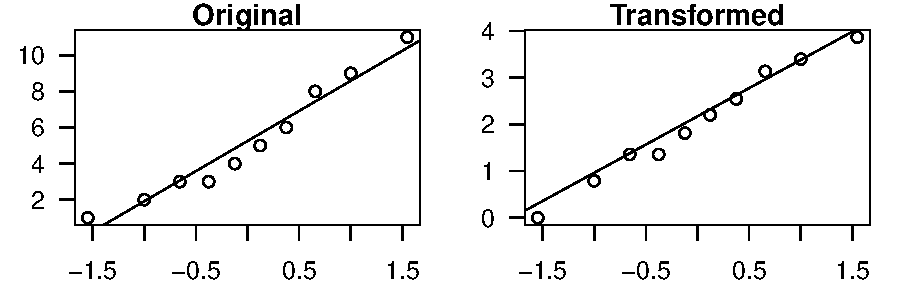
\includegraphics{STAT636_Template-003}
\item Determine the power transformation $\hat{\lambda}_{2}$ that makes the $x_{2}$ values approximately normal. Construct a Q-Q plot for the transformed data.
\begin{Schunk}
\begin{Sinput}
> lambda <- as.numeric(car::powerTransform(used_car[,2])$lambda)
> lambda
\end{Sinput}
\begin{Soutput}
[1] 0.9361967
\end{Soutput}
\begin{Sinput}
> par(mfrow = c(1,2),mar=c(2.5,2.5,1,1))
> qqnorm(used_car[,2], main = "Original", las=1)
> qqline(used_car[,2])
> transformed <- ((used_car[,2] ^ lambda) - 1)/lambda
> qqnorm(transformed, main = "Transformed", las=1)
> qqline(transformed)
\end{Sinput}
\end{Schunk}
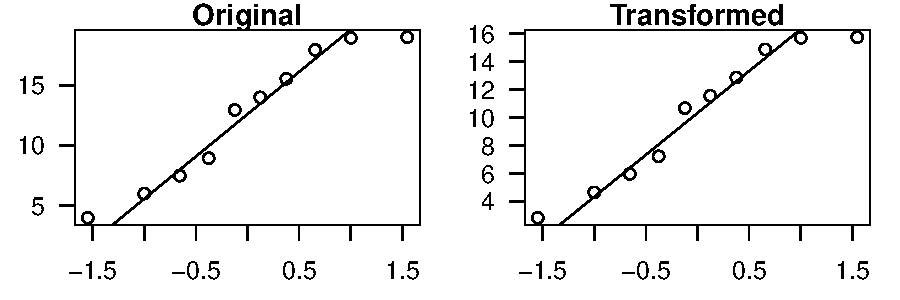
\includegraphics{STAT636_Template-004}
\item Determine the power transformations $\hat{\lambda}' = \left[\hat{\lambda}_{1},\hat{\lambda}_{2}\right]$ that make the $\left[x_{1},x_{2}\right]$ values approximately multivariate normal. Compare the results with those from above.
\begin{Schunk}
\begin{Sinput}
> car::powerTransform(used_car)
\end{Sinput}
\begin{Soutput}
Estimated transformation parameters 
      Age     Price 
1.2732157 0.0310405 
\end{Soutput}
\end{Schunk}
\emph{The values of $\lambda$ required to approximate to the multinormal distribution are different to those computed independently for each variable.}
\end{enumerate}
\item Consider the \texttt{advertising} data. For each of 200 strategies, we have three numeric variables that influence the sales: \texttt{TV}, \texttt{radio}, and \texttt{Newspaper}.
\begin{Schunk}
\begin{Sinput}
> advertising <- read.csv("advertising.csv", row.names = 1)
\end{Sinput}
\end{Schunk}
\begin{enumerate}
\item Construct univariate Q-Q plots for each of the three variables. Also make the three
pairwise scatterplots. Does the multivariate normal assumption seem reasonable?
\begin{Schunk}
\begin{Sinput}
> par(mfrow = c(1,3), mar=c(2.5,2.5,1,1))
> out <- sapply(colnames(advertising[,1:3]), function(x){
+   qqnorm(advertising[,x], main = paste0("Q-Q Plot of ",x), las = 1)
+   qqline(advertising[,x])
+ })
\end{Sinput}
\end{Schunk}
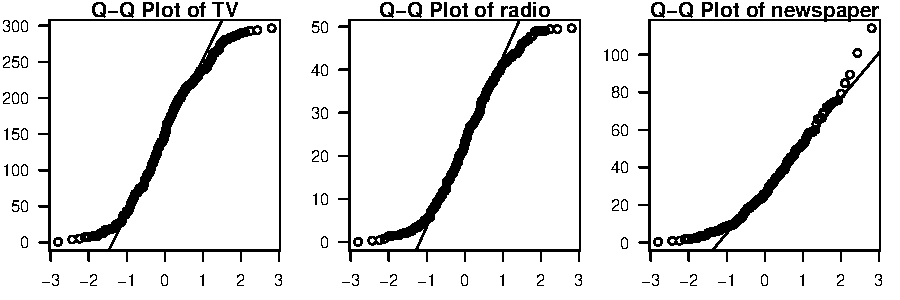
\includegraphics{STAT636_Template-007}
\begin{Schunk}
\begin{Sinput}
> par(mar=c(1,1,1,1))
> plot(advertising[,1:3], las = 1)
\end{Sinput}
\end{Schunk}
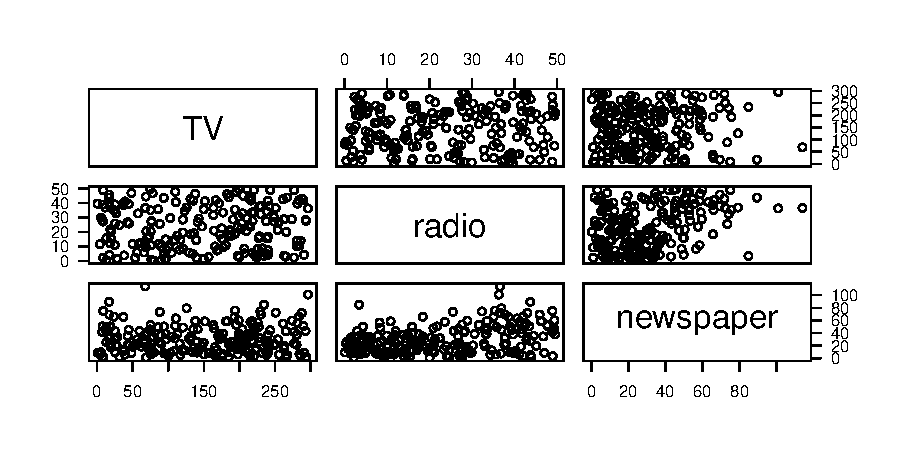
\includegraphics{STAT636_Template-008}

\emph{The multivariable normal distribution does not look reasonable for this dataset because of not all the variables are independently normal}
\item Determine the 95\% confidence ellipsoid for $\mu$. Where is it centered? What are its axes and corresponding half-lengths?
\item Compute 95\% T2 simultaneous confidence intervals for the three mean components.
\item Compute 95\% Bonferroni simultaneous confidence intervals for the three mean components.
\item Carry out a Hotelling's $T^{2}$ test of the null hypothesis H0 : $\mu' = \left[150.0,20.0,30.0\right]$ at $\alpha = 0.05$. What is the test statistic, critical value, and the p-value? What is your conclusion regarding H0?
\item Is $\mu' = [150.0, 20.0, 30.0]$ inside the 95\% confidence ellipse you computed in part (b)? Is this consistent with your findings in part (e)? Hint: It should be.
\item Use the bootstrap to test the same null hypothesis as in part (e), now using this as your test statistic
\[\Lambda = \left(\frac{\left|S\right|}{\left|S_{0}\right|}\right)^{n/2},\]where \[S = \frac{1}{n-1}\sum_{j=1}^{n}(x_{j}-\bar{x})(x_{j}-\bar{x})'\] is the sample covariance matrix, and \[S_{0} = \frac{1}{n-1}\sum_{j=1}^{n}(x_{j}-\bar{x})(x_{j}-\bar{x})'\] is the sample covariance matrix under the assumption that $H_{0}$ is true. So that all our answers match, first do \texttt{set.seed(2)}, and use $B=500$ bootstrap iterations. What is the p-value?
\begin{Schunk}
\begin{Sinput}
> 
\end{Sinput}
\end{Schunk}
\end{enumerate}
\end{enumerate}
\end{document}
